\documentclass[10pt,a5]{article}

\usepackage{paracol}
%\usepackage[landscape]{geometry}
\usepackage[left=1.5cm, right=1.5cm, top = 2cm, bottom = 2cm]{geometry}
%\usepackage{pdfpages}
\usepackage{graphicx}
\usepackage{liturg}
\usepackage{lipsum}

\begin{document}

\massenglish

%\psalmheading{Psalm 42---Judica me}

%\instruct{The priest, signing himself with the Sign of the Cross, says:}

%\leslettrine{C}onf'iteor Deo omnipot'enti, be'at"ae Mar'i"ae semper
%V'irgini, be'ato Micha'eli Arch'angelo, be'ato Jo'anni Bapt'ist"ae,
%sanctis Ap'ostolis Petro et Paulo, 'omnibus Sanctis, et tibi Pater:
%quia pecc'avi nimis congitati'one, verbo, et 'opere:

\begin{paracol}{2}

\section*{Introductory Rites}

\subsection*{Entrance}

\subsection*{Greeting}

\switchcolumn

\section*{Acolhida}

\switchcolumn

\priest{The Lord be with you}
\server{And with your spirit}

\switchcolumn

\padre{A graça de Nosso Senhor Jesus Cristo, o amor do Pai e a comunhão do Espírito Santo estejam convosco.}
\todos{Bendito seja Deus, que nos reuniu no amor de Cristo.}

\switchcolumn*

\subsection*{Penitential Act}

\switchcolumn

\subsection*{Ato Penitencial}

\switchcolumn

\end{paracol}

\begin{figure}[h]
	\centering
	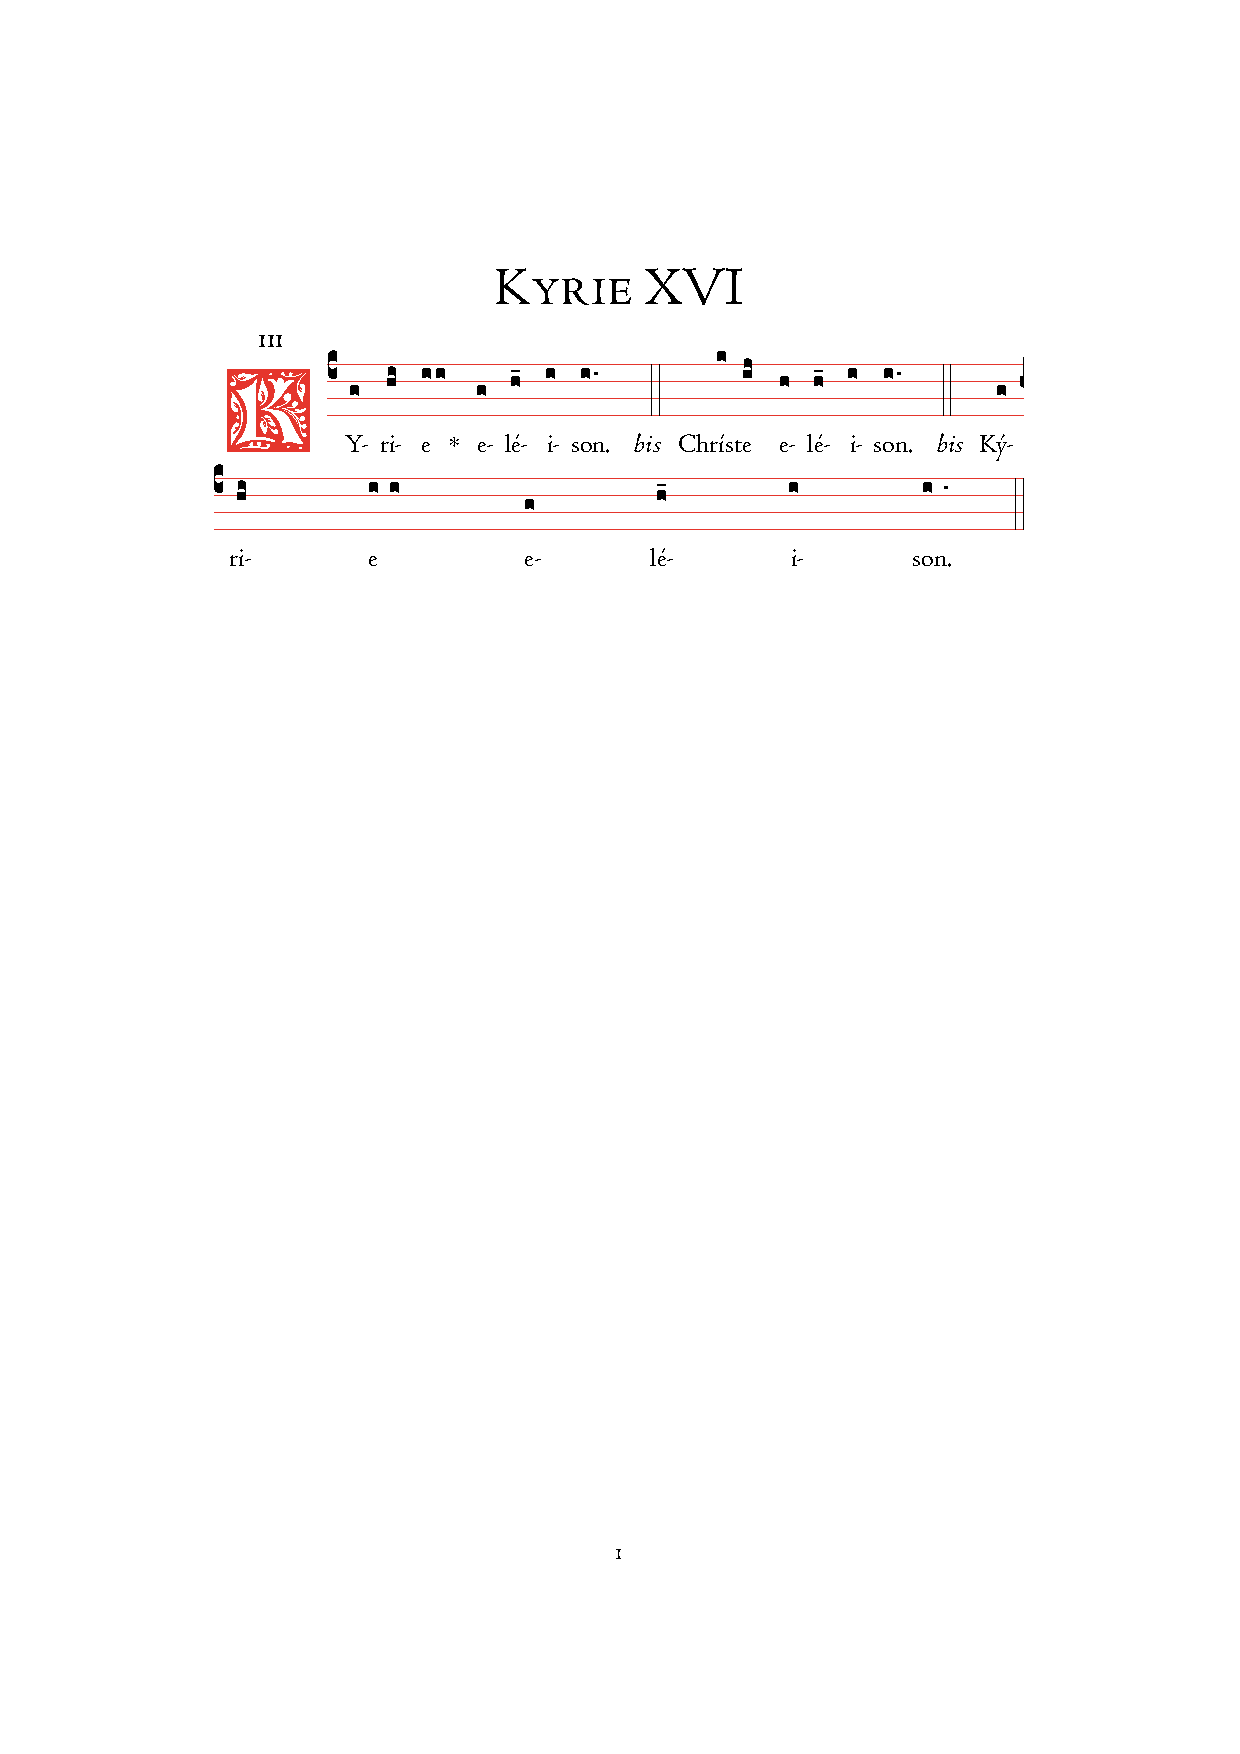
\includegraphics[trim = 35mm 200mm 35.5mm 45mm, clip, width = 0.8\textwidth]{scores/Kyrie-XVI.pdf}
\end{figure}

\begin{paracol}{2}

(Lord, have mercy. Christ, have mercy. Lord, have mercy.)
\switchcolumn
(Senhor, tende piede. Cristo, tende piedade. Senhor, tende piedade)

\switchcolumn*

\subsection*{Glory to God}

\switchcolumn

\subsection*{Gl\'oria}

\end{paracol}

\begin{figure}
	\centering
	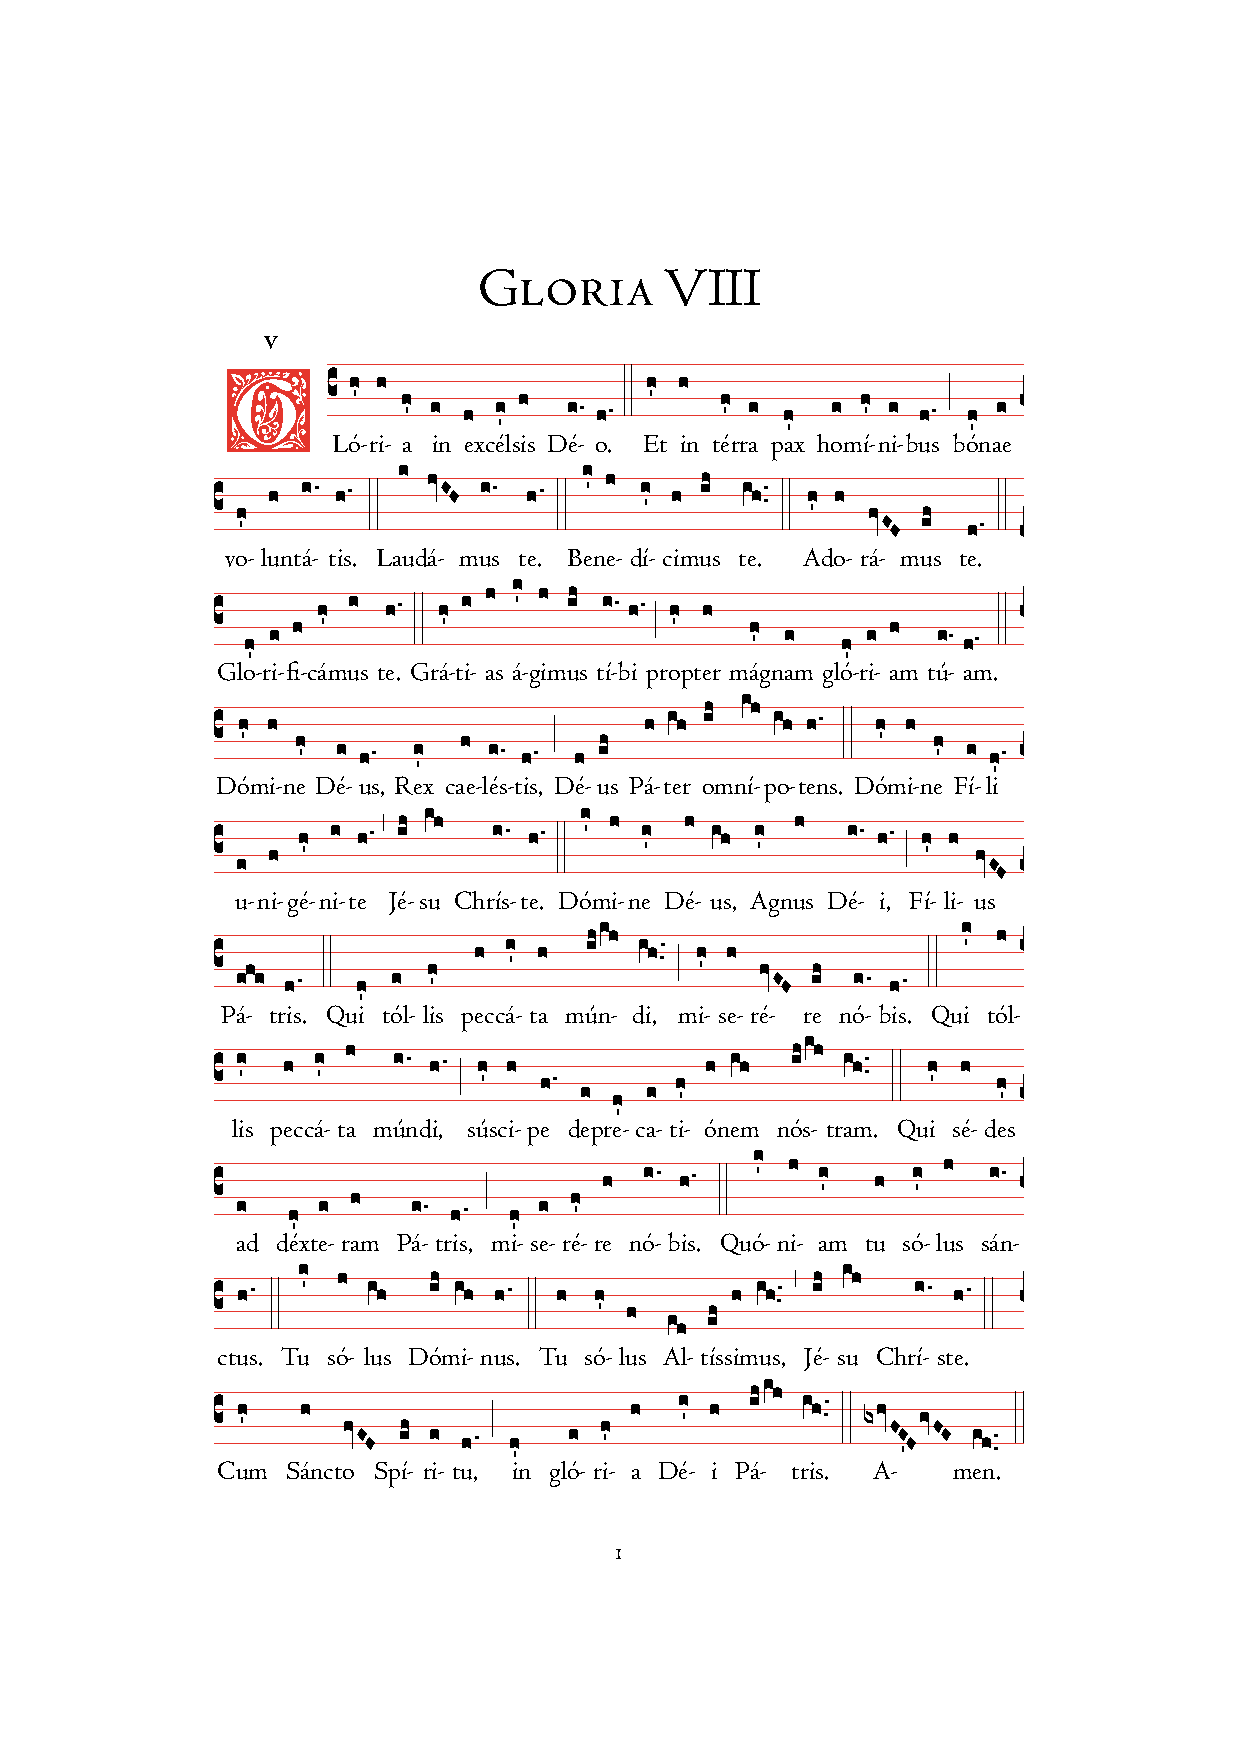
\includegraphics[trim = 35mm 45mm 35.5mm 45mm, clip, width = 0.8\textwidth]{scores/Gloria-VIII.pdf}
\end{figure}

\begin{paracol}{2}

(Glory to God in the highest,
and on earth peace to people
of good will.
We praise you, we bless you,
we adore you, we glorify you,
we give you thanks for your great
glory,
Lord God, heavenly King, O God,
almighty Father.
Lord Jesus Christ, Only Begotten Son,
Lord God, Lamb of God, Son of the
Father,
you take away the sins of the world,
have mercy on us;
you take away the sins of the world,
receive our prayer;
you are seated at the right hand
of the Father, have mercy on us.
For you alone are the Holy One,
you alone are the Lord,
you alone are the Most High,
Jesus Christ, with the Holy Spirit,
in the glory of God the Father. Amen.)

\switchcolumn

(Gl\'oria a Deus nas alturas e paz na terra aos homens por Ele amados.
 Senhor Deus, Rei dos c\'eus, Deus Pai todo-poderoso:
 n\'os Vos louvamos, n\'os Vos bendizemos, n\'os Vos adoramos, n\'os Vos glorificamos,
 n\'os Vos damos graças, por vossa imensa gl\'oria.
 Senhor Jesus Cristo, Filho Unig\'enito, Senhor Deus, Cordeiro de Deus, Filho de Deus Pai:
 V\'os que tirais o pecado do mundo, tende piedade de n\'os;
 V\'os que tirais o pecado do mundo, acolhei a nossa súplica;
 V\'os que estais \`a direita do Pai, tende piedade de n\'os.
 S\'o V\'os sois o Santo;
 s\'o V\'os, o Senhor;
 s\'o V\'os, o Altíssimo, Jesus Cristo;
 com o Espírito Santo na gl\'oria de Deus Pai.
 Am\'em)

 \switchcolumn*

 \section*{Litugy of the Word}

 \subsection*{First Reading}

 \lipsum[3]

 \switchcolumn

 \section*{Liturgia da Palavra}

 \subsection*{Primeira Leitura}

 \lipsum[3]

\end{paracol}

%\greatfeast{Feria Quinta in Cena Domini}{I}

%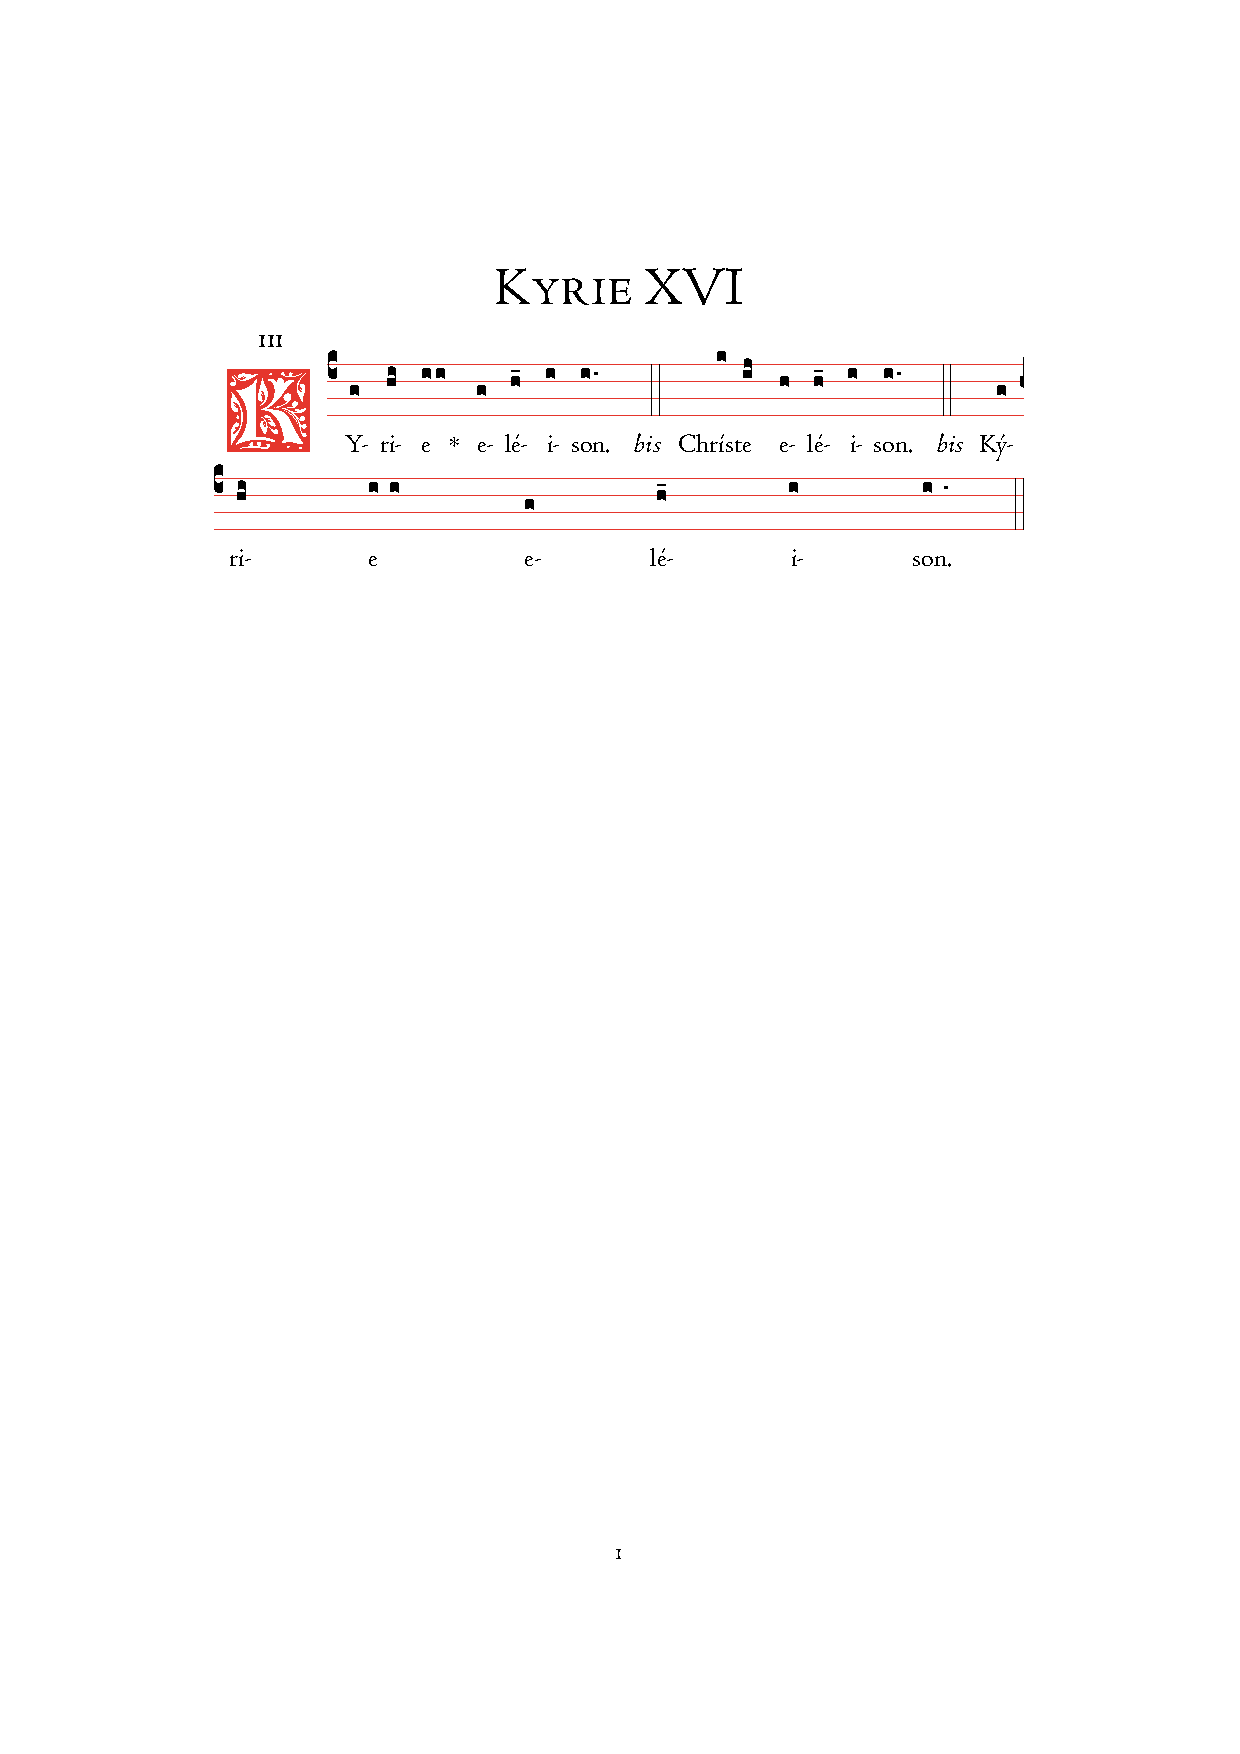
\includepdf[pages=-,pagecommand={},width=\textwidth, trim = 35mm 200mm 20mm 45mm, clip]{scores/Kyrie-XVI.pdf}
\end{document}
